\documentclass[12pt]{article}

% ── Page geometry (Letter, 1-inch margins matching the Word template) ──
\usepackage[letterpaper, margin=1in]{geometry}

% ── Font Configuration ──
\usepackage[T1]{fontenc}

% ── Packages ──
\usepackage{array}      % better table columns
\usepackage{graphicx}   % images
\usepackage{xcolor}     % colors
\usepackage{enumitem}   % list customization
\usepackage{hyperref}   % clickable links (optional)
\usepackage{tabularx}   % full-width tables
\usepackage{setspace}   % line spacing
\usepackage{listings}   
\usepackage{amsmath}
\usepackage{float}


\definecolor{codebg}{rgb}{0.96,0.96,0.94}

\lstset{
    backgroundcolor=\color{codebg},
    basicstyle=\ttfamily\footnotesize,
    keywordstyle=\color{magenta},
    numberstyle=\tiny\color{gray},
    numbers=left,
    numbersep=8pt,
    frame=none,
    breaklines=true,
    showstringspaces=false,
    tabsize=4,
    xleftmargin=1.5em,
    aboveskip=10pt,
    belowskip=10pt,
}
\usepackage{fancyhdr}
\pagestyle{fancy}
\fancyhf{} % Clears default header and footer settings

% Define your top header elements
\lhead{Tel Aviv University}
\rhead{FPGA Stopwatch Lab}

% Define your bottom footer element (Centered Page Numbering)
\cfoot{\thepage}

% Adjust the thickness of your top header line
\renewcommand{\headrulewidth}{0.4pt}
\begin{document}

% �� ── Custom Title Page ──
\begin{titlepage}
\begin{center}
    % 1. University Logo Centered at Top-Middle
    
\includegraphics[width=0.35\textwidth]{Tel_Aviv_university_logo_-_English.png} 
    \vspace{2cm}
    
    % 2. Faculty Name
    {\large \textbf{The Iby and Aladar Fleischman Faculty of Engineering}} \\
    \vspace{0.6cm}
    
    % 3. Lab Name
    {\large \textbf{Electronics - Laboratory B}} \\
    \vfill 
    
    % 4. Main Title Framed with Thicker Horizontal Lines
    \rule{\linewidth}{2.5pt} \\ [0.5cm]
    {\huge \textbf{FPGA Experiment Report - Stopwatch}} \\ [0.3cm]
    \rule{\linewidth}{2.5pt} \\
    \vfill 
    
    % 5. Student Details (Centered & Underlined IDs)
    \textbf{Student 1:} \\
    Name: Mahmoud Stitia \\
    ID: \underline{214032682} \\
    \vspace{1cm} 
    
    \textbf{Student 2:} \\
    Name: Jihad Abu Daya \\
    ID: \underline{318791068}
    
\end{center}
\end{titlepage}
\newpage
\pagenumbering{arabic} % Starts numbering from 1 on this page

\renewcommand{\contentsname}{Table of Contents}
\tableofcontents % This automatically generates your entire page-tracked grid!
\newpage

% =========================================================================
% ── NEW SECTION: Part 1 - Full Adder (FA) ──
% =========================================================================
\section{Full Adder (FA)}

% ── Subtitle 1.1 ──
\subsection{Truth Table}


\noindent \textbf{Question:} Write the truth table for the Full Adder, showing inputs a, b, ci and outputs sum, co. Which rows produce a carry out?

\begin{table}[h!] % �� Added [h!] here to force the table to stay in place
    \centering
    \begin{tabular}{|c|c|c||c|c|}
        \hline
        \textbf{a} & \textbf{b} & \textbf{ci} & \textbf{sum} & \textbf{co} \\ \hline
        0 & 0 & 0 & 0 & 0 \\ \hline
        0 & 0 & 1 & 1 & 0 \\ \hline
        0 & 1 & 0 & 1 & 0 \\ \hline
        0 & 1 & 1 & 0 & 1 \\ \hline
        1 & 0 & 0 & 1 & 0 \\ \hline
        1 & 0 & 1 & 0 & 1 \\ \hline
        1 & 1 & 0 & 0 & 1 \\ \hline
        1 & 1 & 1 & 1 & 1 \\ \hline
    \end{tabular}
    \caption{Full Adder Truth Table}
\end{table}

\vspace{1cm}
\noindent \textbf{Rows that produce carry out:} Rows with at least two 1's in the input will indeed produce a high carry out, as we can tell from the table when looking at lines number 4,6,7,8.

\vspace{0.2cm} % Creates blank layout space on the page


% ── Subtitle 1.2 ──
\subsection{Gate-Level Schematic}
\noindent \textbf{Question:} Draw a schematic showing only AND, OR, XOR gates that implement your FA.

\begin{figure}[h]
    \centering
    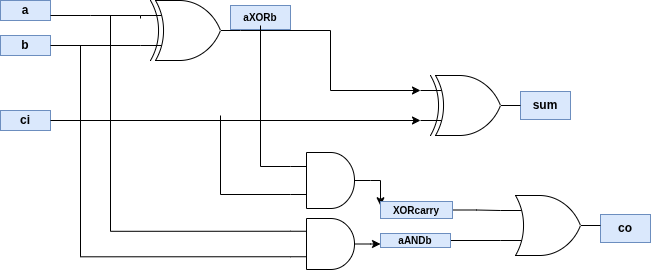
\includegraphics[width=1\linewidth]{full_adder.drawio.png}
    \caption{Full Adder Gate-Level Schematic}
    \label{fig:full_adder_schematic}
\end{figure}

% ── Subtitle 1.3 ──
\subsection{Waveform Simulations}
\noindent \textbf{Question:} Provide an annotated waveform of your simulation.
\begin{figure}[h]
    \centering
    % You can use cm, in, or pt for the height
    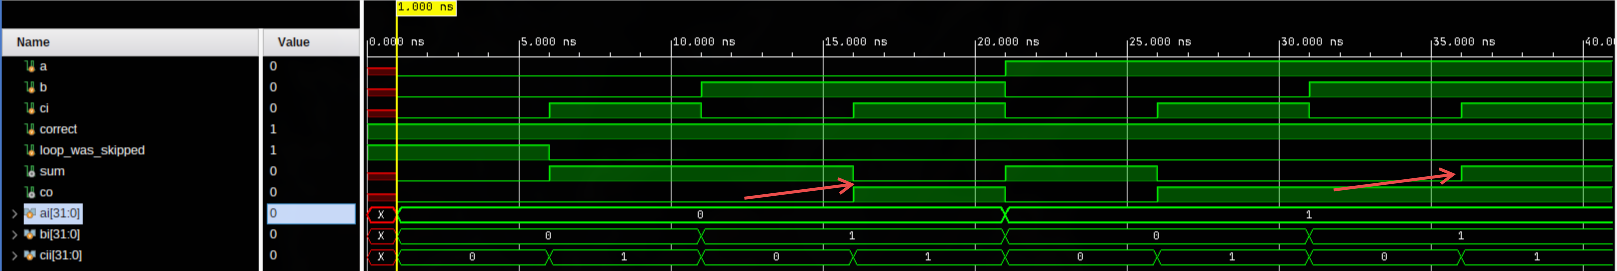
\includegraphics[width=\textwidth, height=5cm]{FA_wave.png} 
    \caption{Detailed view of the Full Adder simulation.}
    \label{fig:fa_annotated}
\end{figure}

\noindent \textbf{Explanation of the waveform:}
First of all, as we can see, correct stayed at ’1’ for the whole duration of the simulation indicating that the FA is working as intended.
The first line represents the value of ``a''. 
The second line represents the value of ``b''. 
The third line represents the value of ``ci'' . 
The fourth and fifth lines represent the values of ``correct'' and ``loop\_was\_skipped''.\\ We use these two values to verify whether our calculation is correct. 
The bottom two lines represent the value of ``sum'' and the value of ``co'' (carry-out) respectively; these values are the final outputs from our design where:
\vspace{0.1 cm}
\begin{itemize}
    \item \textbf{i:} The first red arrow points to the transition at 15 ns. At this moment, the input ci switches from 0 to 1, while a and b remain at 0. This results in a total sum of 1. Consequently, the sum output changes from 0 to 1 to reflect this addition.
    \item \textbf{ii:} he second red arrow illustrates the transition at 35 ns. At this point, the input a is 1, b is 0, and ci switches from 0 back to 1. Because the sum of equals 2 (represented as binary 10), the sum bit drops back to 0. Simultaneously, the arrow indicates that co (carry out) transitions from 0 to 1 to represent the carry bit.
\end{itemize}

\vspace{4cm} % Creates blank layout space on the page
\newpage


% =========================================================================
% ──  Section 2 - Conditional Sum Adder (CSA)─
% =========================================================================
\section{Conditional Sum Adder (CSA(N))}

% =========================================================================
% ──  Sub-section 2.1 - Conditional Sum Adder (CSA)─
\subsection{Block Diagram}
\noindent \textbf{Question:} Design a block diagram for the module, use instantiated modules, show and explain any other logic necessary.

\begin{figure}[h]
    \centering
    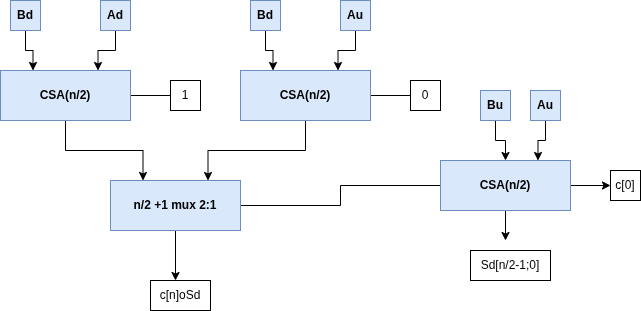
\includegraphics[width=1\linewidth]{CSA.png}
    \caption{CSA Block Diagram}
    \label{fig:placeholder}
\end{figure}

\noindent \textbf{Block Diagram Explanation:} This is the classic CSA block diagram that we have
seen in the course "Digital Logic Systems".\\ It adds parallelism to the addition operation,
which therefor makes the addition operation much faster, but this great advantage of speed comes at the cost of space. 
How it works and where is the quick part?
When adding two numbers each of length of more than a single bit, in order to compute the result for each two added bits, one must include in the addition the carry bit that generated from adding the two previous bits, the problem emerges from the fact that the carry bit is not ready yet.  For the desired carry bit to be ready, the two current bits should "wait for it" to be calculated after a series of sequential addition that should have taken place previously. which results in slowing down the addition speed (like the Ripple Carry Adder for example), so alternatively, the CSA suggests to calculate all the addition operations in advance twice, once assuming $c_i = 0$ and once assuming $c_i = 1$. 
At the end, the correct result is chosen using a multiplexer with the select bit being the $c_o$ output-bit of the CSA that just finished adding the two right-hand side parts of the two bit string inputs.
This design is recursive, with CSA(1) being the FA module we designed earlier.\\\vspace{0.1 cm}

% =========================================================================
% ── Sub-section 2.2 - Time Comparison with Ripple Carry Adder ─
\subsection{Time Comparison with Ripple Carry Adder}


\noindent \textbf{Question:} How does the Conditional Sum Adder improve timing compared to a simple ripple-carry adder? In what situations would a ripple-carry adder still be preferable?\\\\

\noindent \textbf{Answer} the CSA improves timing by eliminating the full $N$-bit carry ripple. By precomputing MSB-side sums for both possible carry-in values $c_i = 0$ and $c_i = 1$, the circuit only awaits the lower-block carry to select the result via multiplexers. Consequently, the worst-case delay is reduced to the lower-block carry generation plus the MUX chain delay, rather than a full $N$-stage propagation.\\
A ripple-carry adder is still preferable when area, power, and simplicity are more important than speed. For small bit-widths the ripple delay is probably acceptable, so the extra duplicated logic and multiplexers of a CSA are not worth the cost. RCAs are also attractive in low-power/low-area designs and in non-critical timing paths, since they have minimal hardware, lower switching activity, and are easier to implement and verify.

% =========================================================================
% ──  Sub-section 2.3 - Generate Block ─

\subsection{Generate Block}

\noindent \textbf{Question:} What is a "generate block"? Why do we need to use it in the CSA implementation?\\\\
\noindent \textbf{Answer} A generate block in Verilog is an elaboration-time construct (using
generate/endgenerate with for/if/case) that lets the compiler replicate or conditionally include hardware based on parameters or constants. We need it in the CSA because
the adder is built from repeated bit-slices/blocks. Instead of manually instantiating the same logic N times, a
generate loop creates these repeated instances parameterically, making the design scalable.
to any bit-width and consistent across all stages \\\\

% =========================================================================
% ──  Sub-section 2.4 - Simulation Waveform - CSA(3) ─

\subsection{Simulation Waveform - CSA(3)}
\noindent \textbf{Question:}Provide an annotated waveform of your simulation. How can you confirm from the waveform that the "conditional" part of the design works correctly?\\\\
\begin{figure}[H]
    \centering
    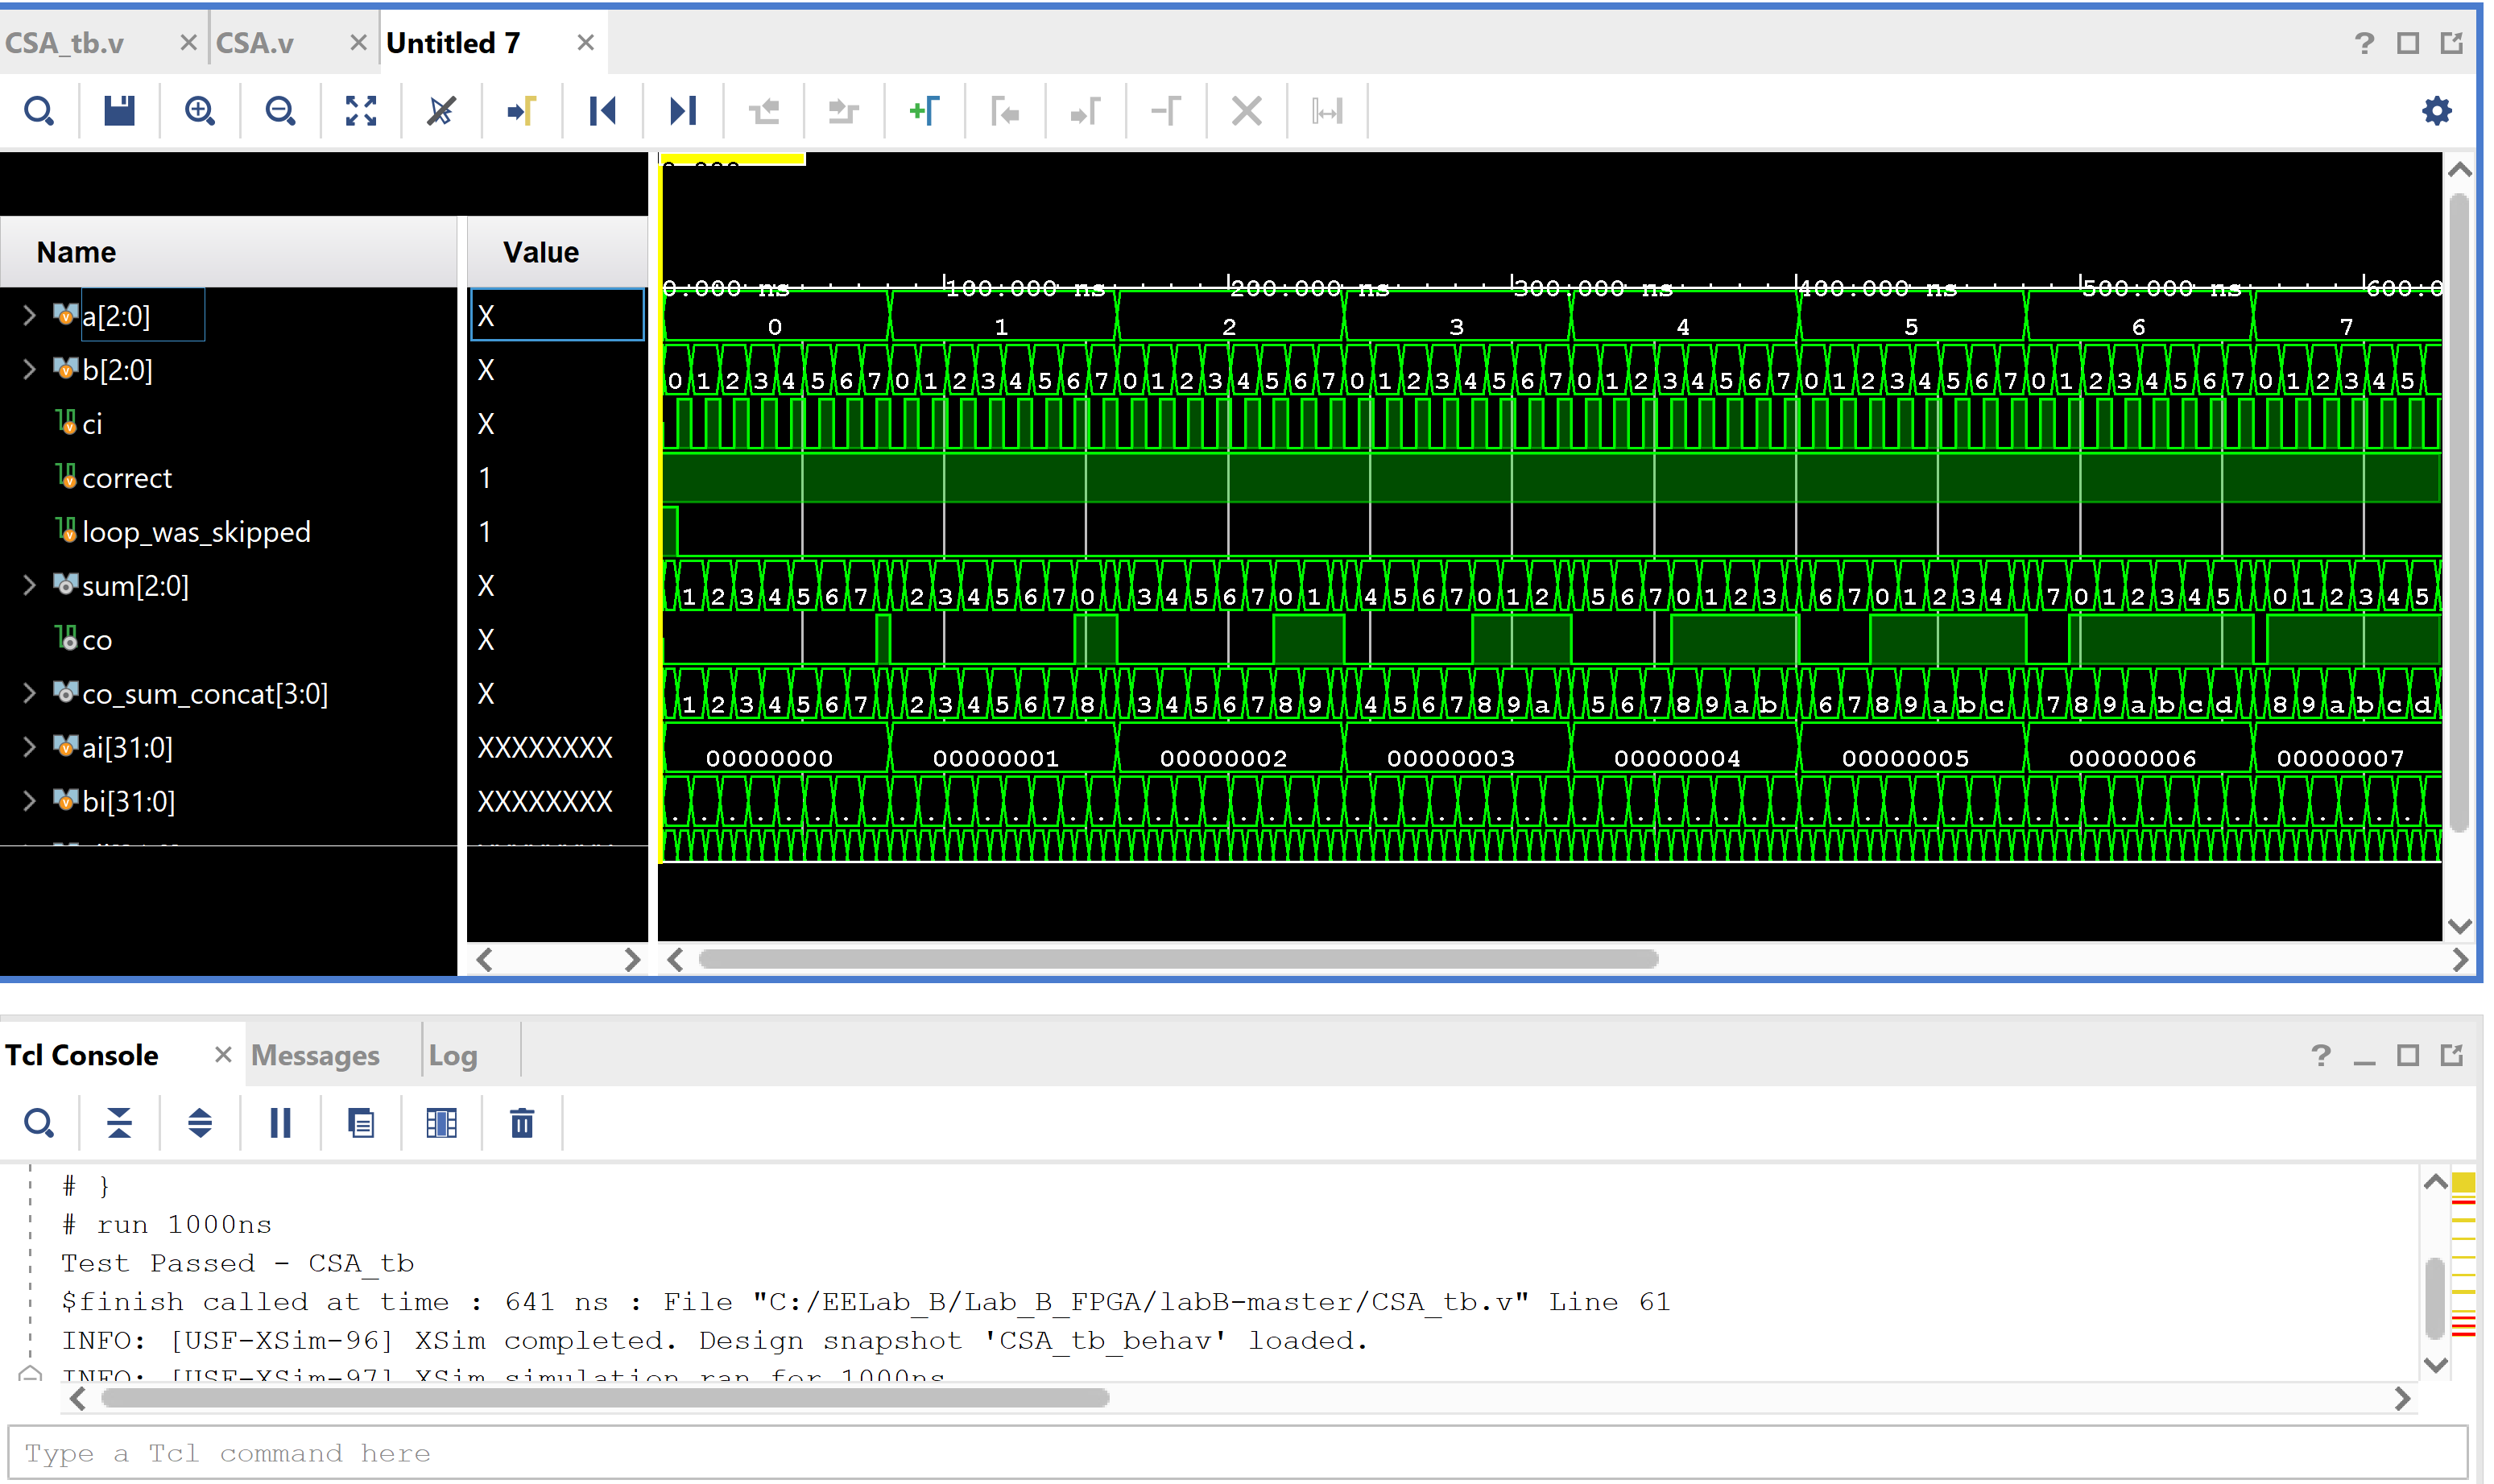
\includegraphics[width=1\linewidth]{CSA(3)full_wave.png}
    \caption{CSA(3) Simulation Waveform - Full Simulation}
    \label{fig:placeholder_csa(fignumber4)}
\end{figure}
\noindent The simulation of the CSA(3) indeed secceeded and we got a "Test Passed - CSA-tb" message in the TCL console, also another point that worth mentioning here as it is visible from the waveform that the correct signal remained in "high" throughout the entire simulatoion time which is another indicator of success.
\begin{figure}[H]
    \centering
    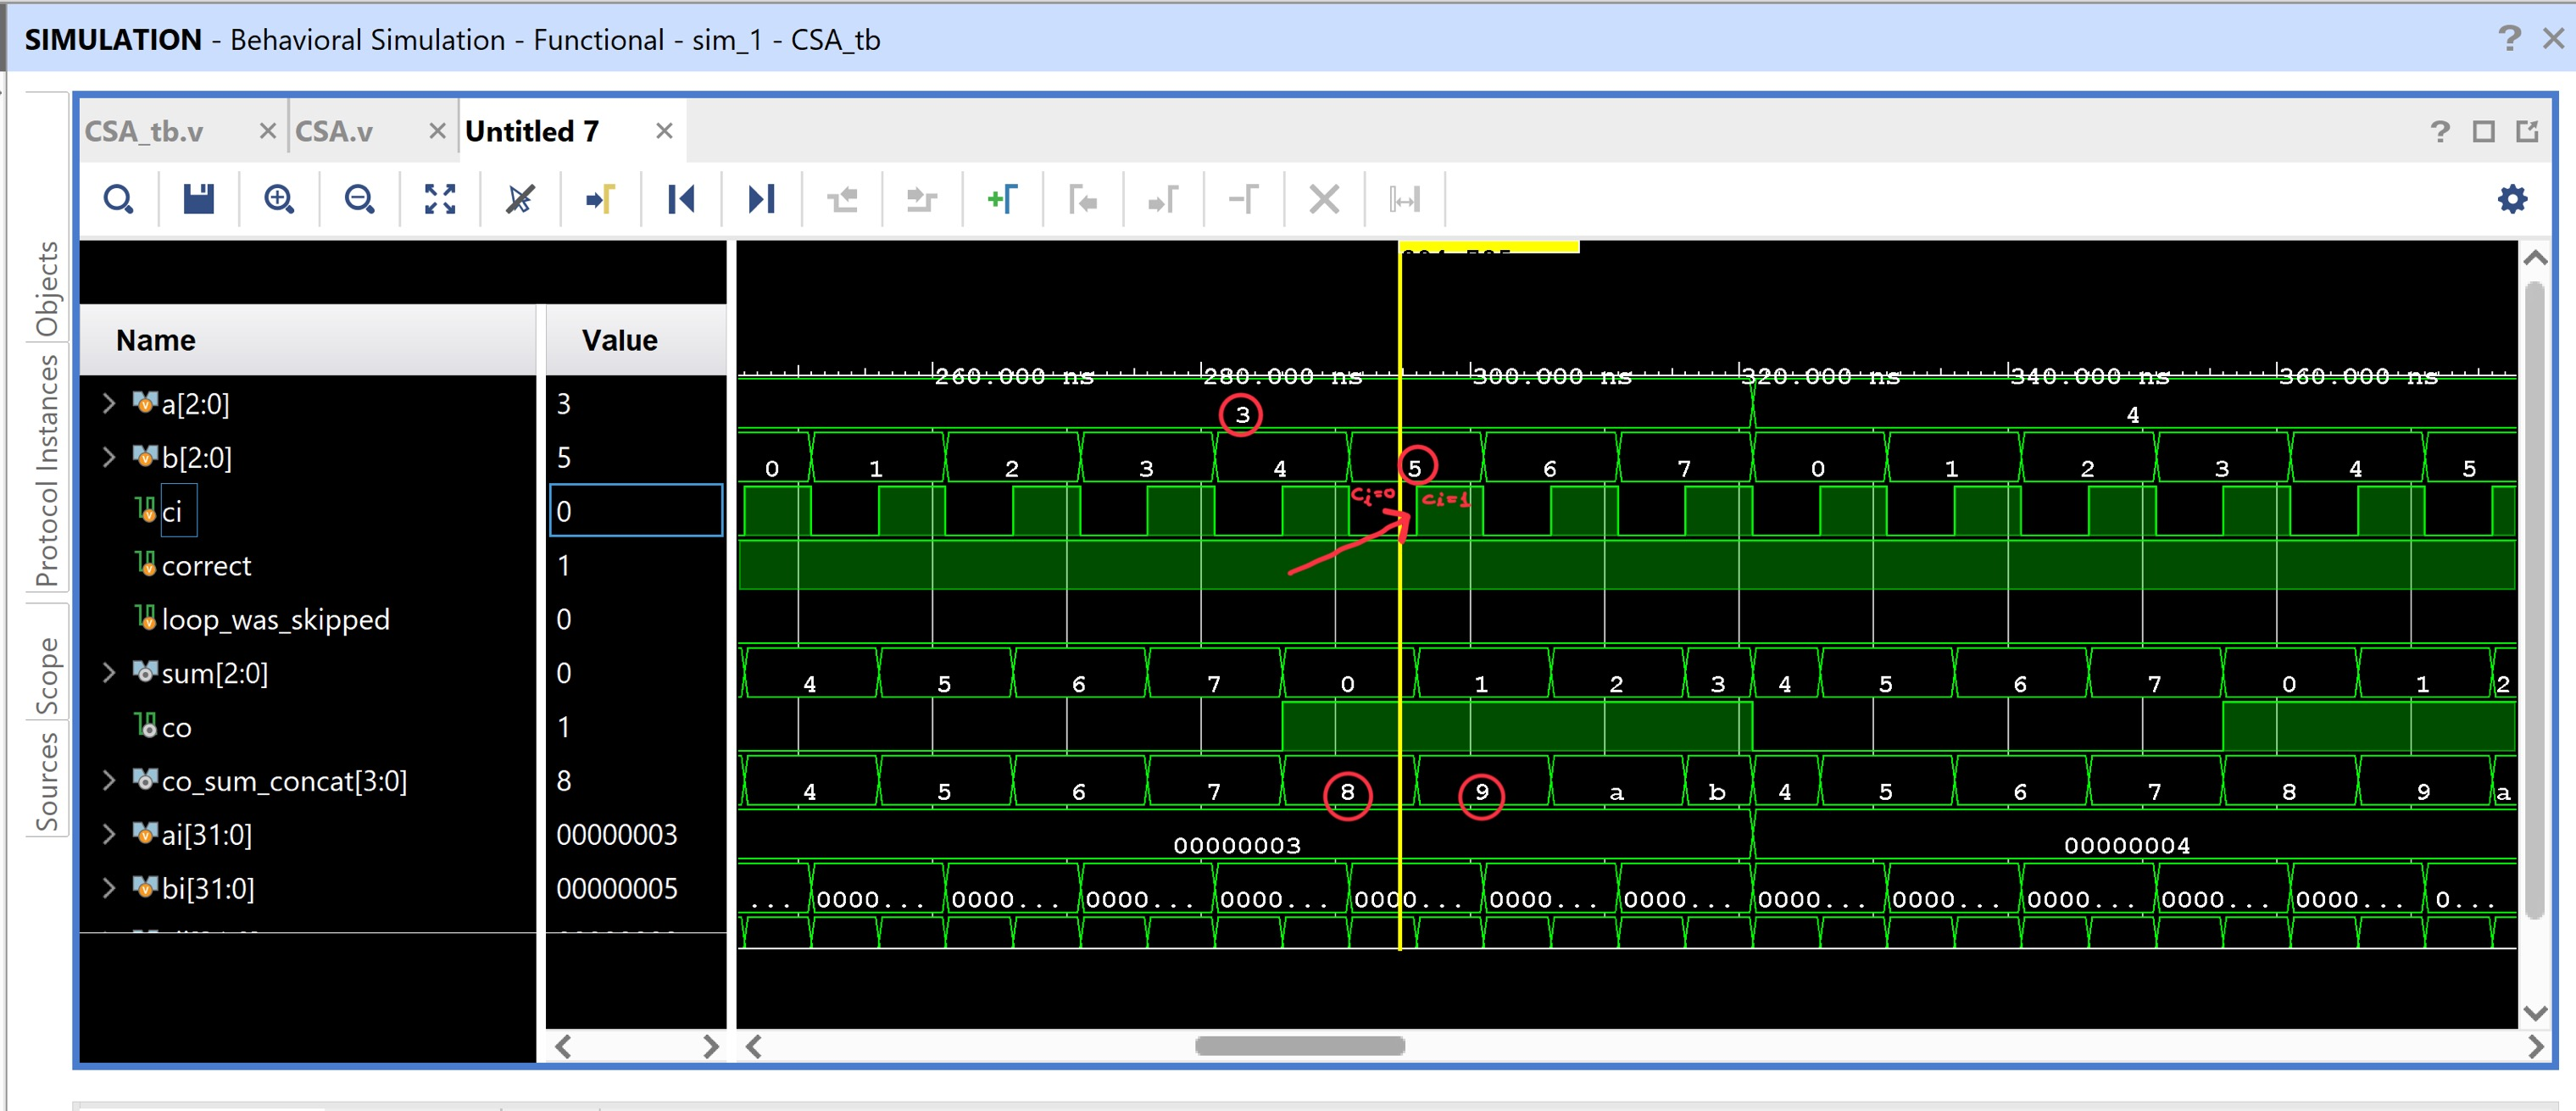
\includegraphics[width=1\linewidth]{CSA3-Annotated.jpg}
    \caption{CSA(3) Simulation Waveform (Annotated))}
    \label{fig:placeholder_csa(fignumber5)}
\end{figure}
%
% I should add here the CSA(3) Annotated 2
%
% Which must be Figure - 6

%%%%%%%%%%%%%%%%%%%%%%%%%%%%%%%

% ──  Sub-section 2.5 - Simulation Waveform - CSA(4) ─

\subsection{Simulation Waveform - CSA(4)}
\noindent \textbf{Refering to the previous section} Revisiting the previous section but this time with the parameter N set to 4 in the CSA implementation, and the parameter Width set to 4 in the CSA-testbench.\\

\begin{figure}[H]
    \centering
    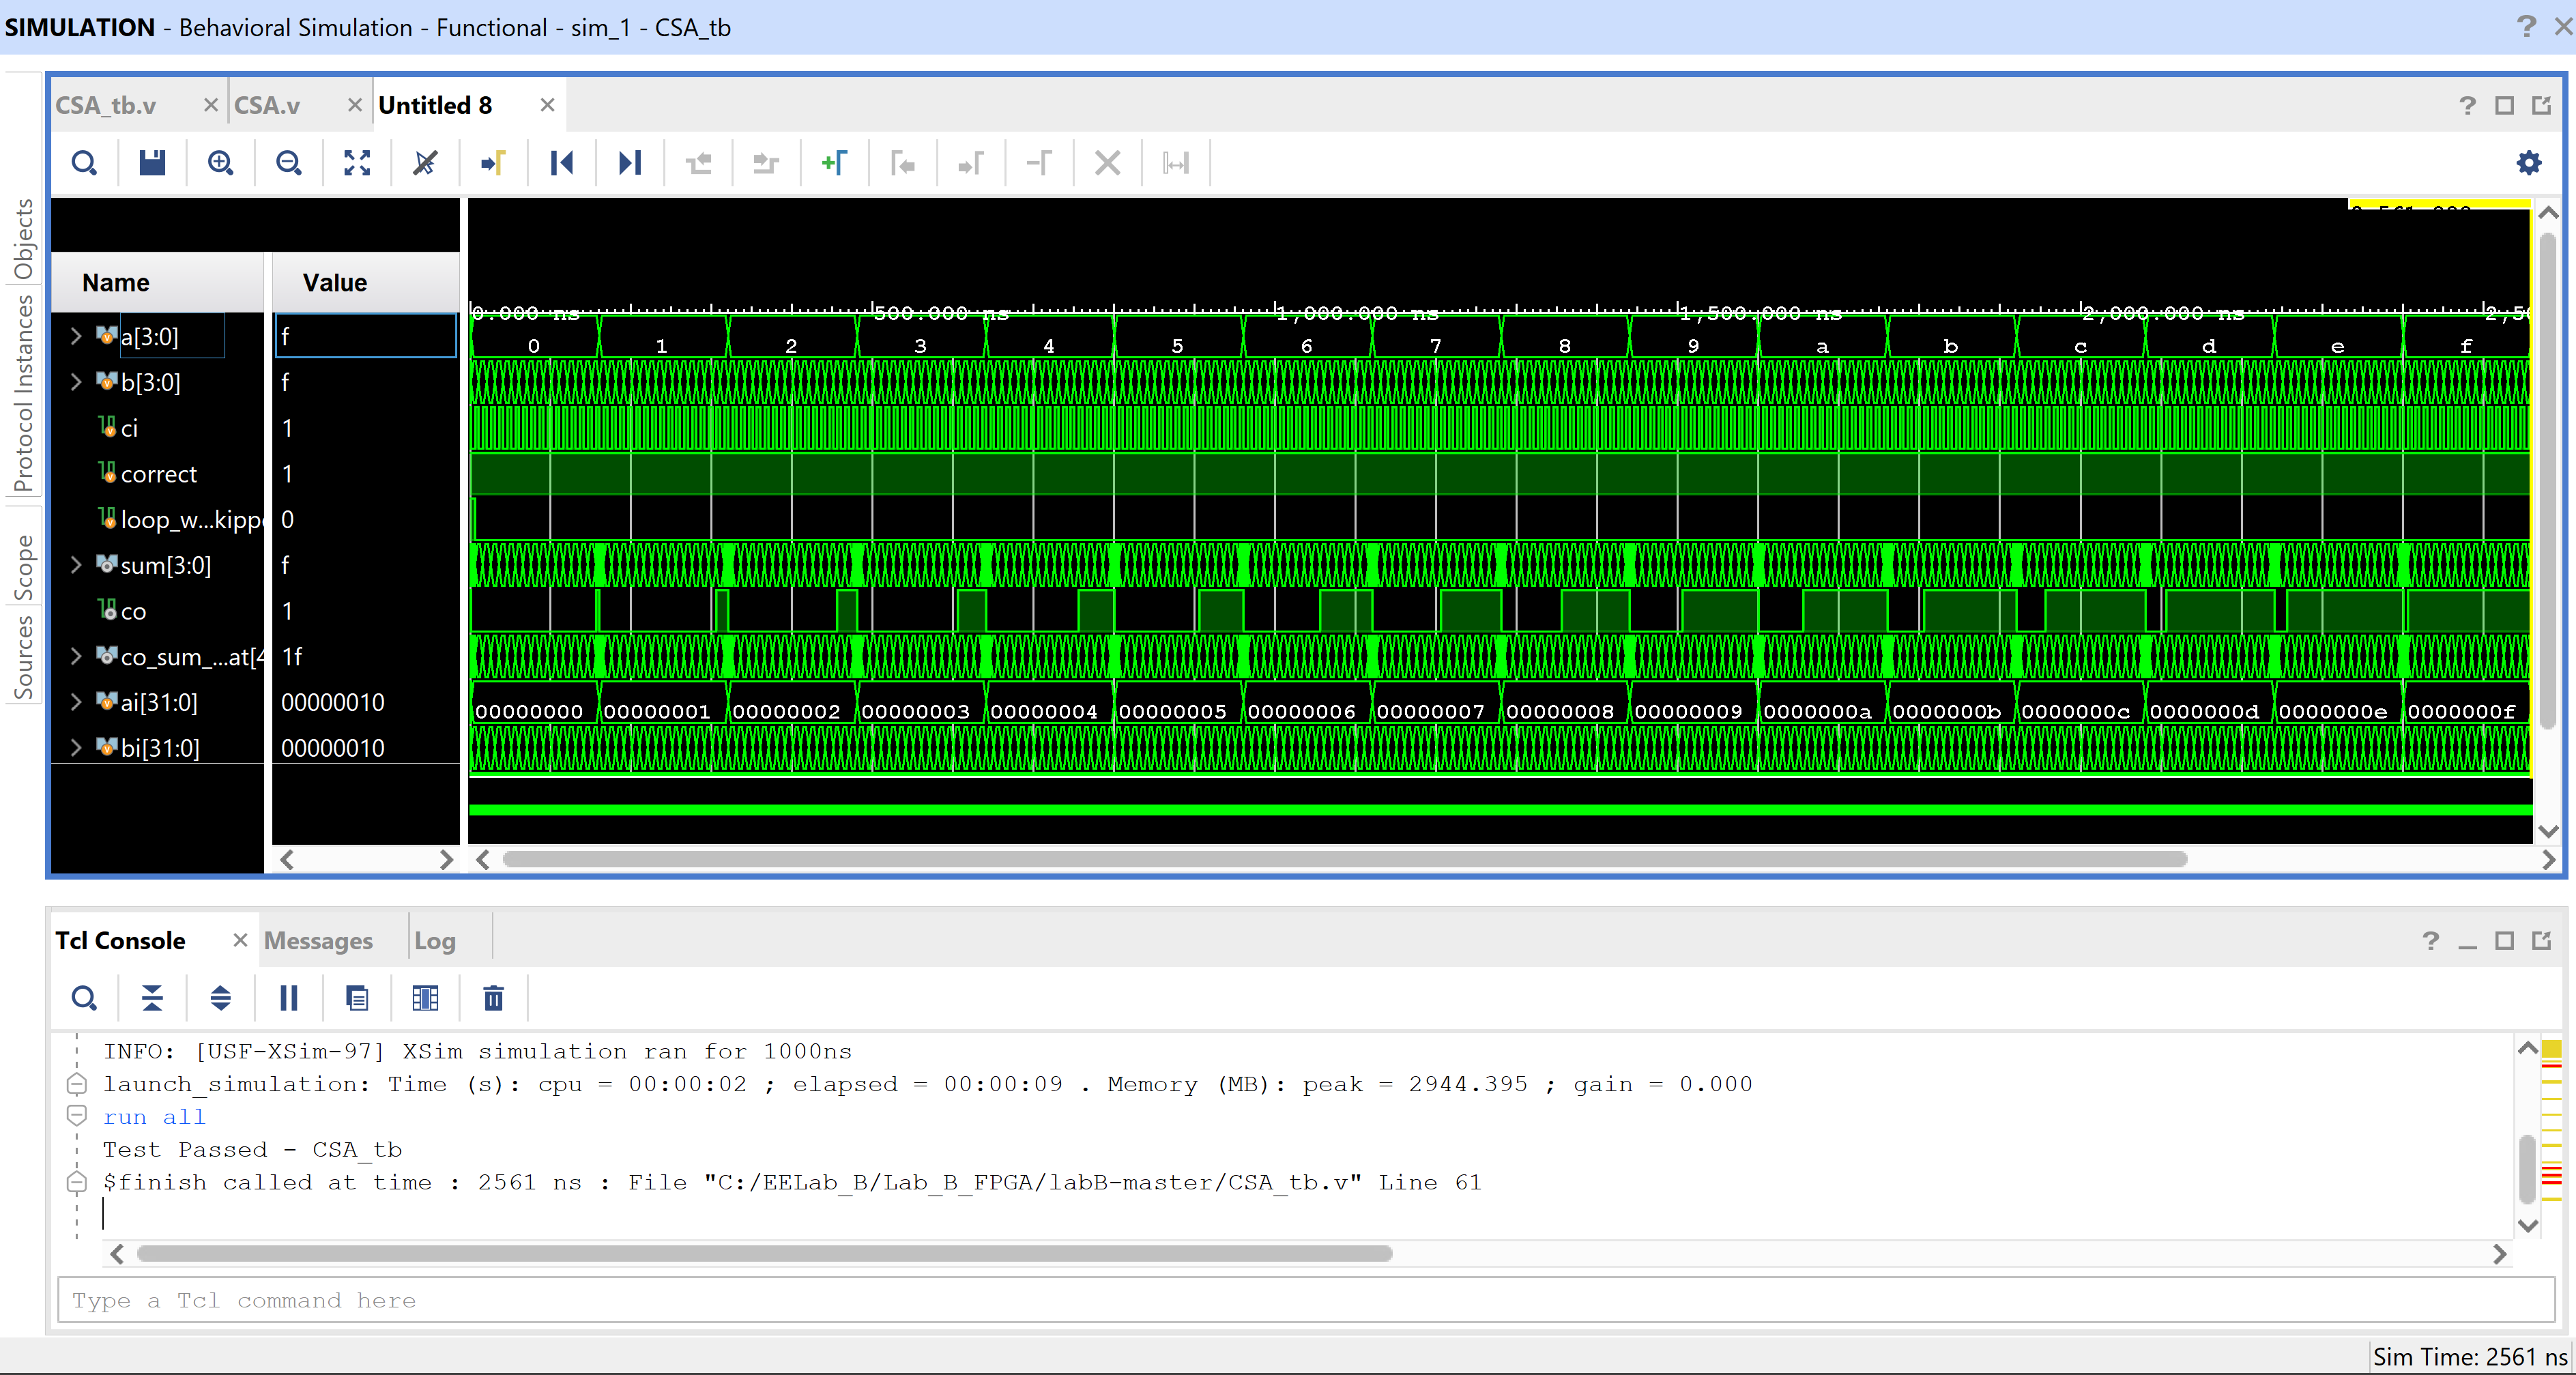
\includegraphics[width=1\linewidth]{CSA(4)FullWF.png}
    \caption{CSA(4) Simulation Waveform - Full Simulation}
    \label{fig:placeholder_csa(fignumber7)}
\end{figure}

\begin{figure}[H]
    \centering
    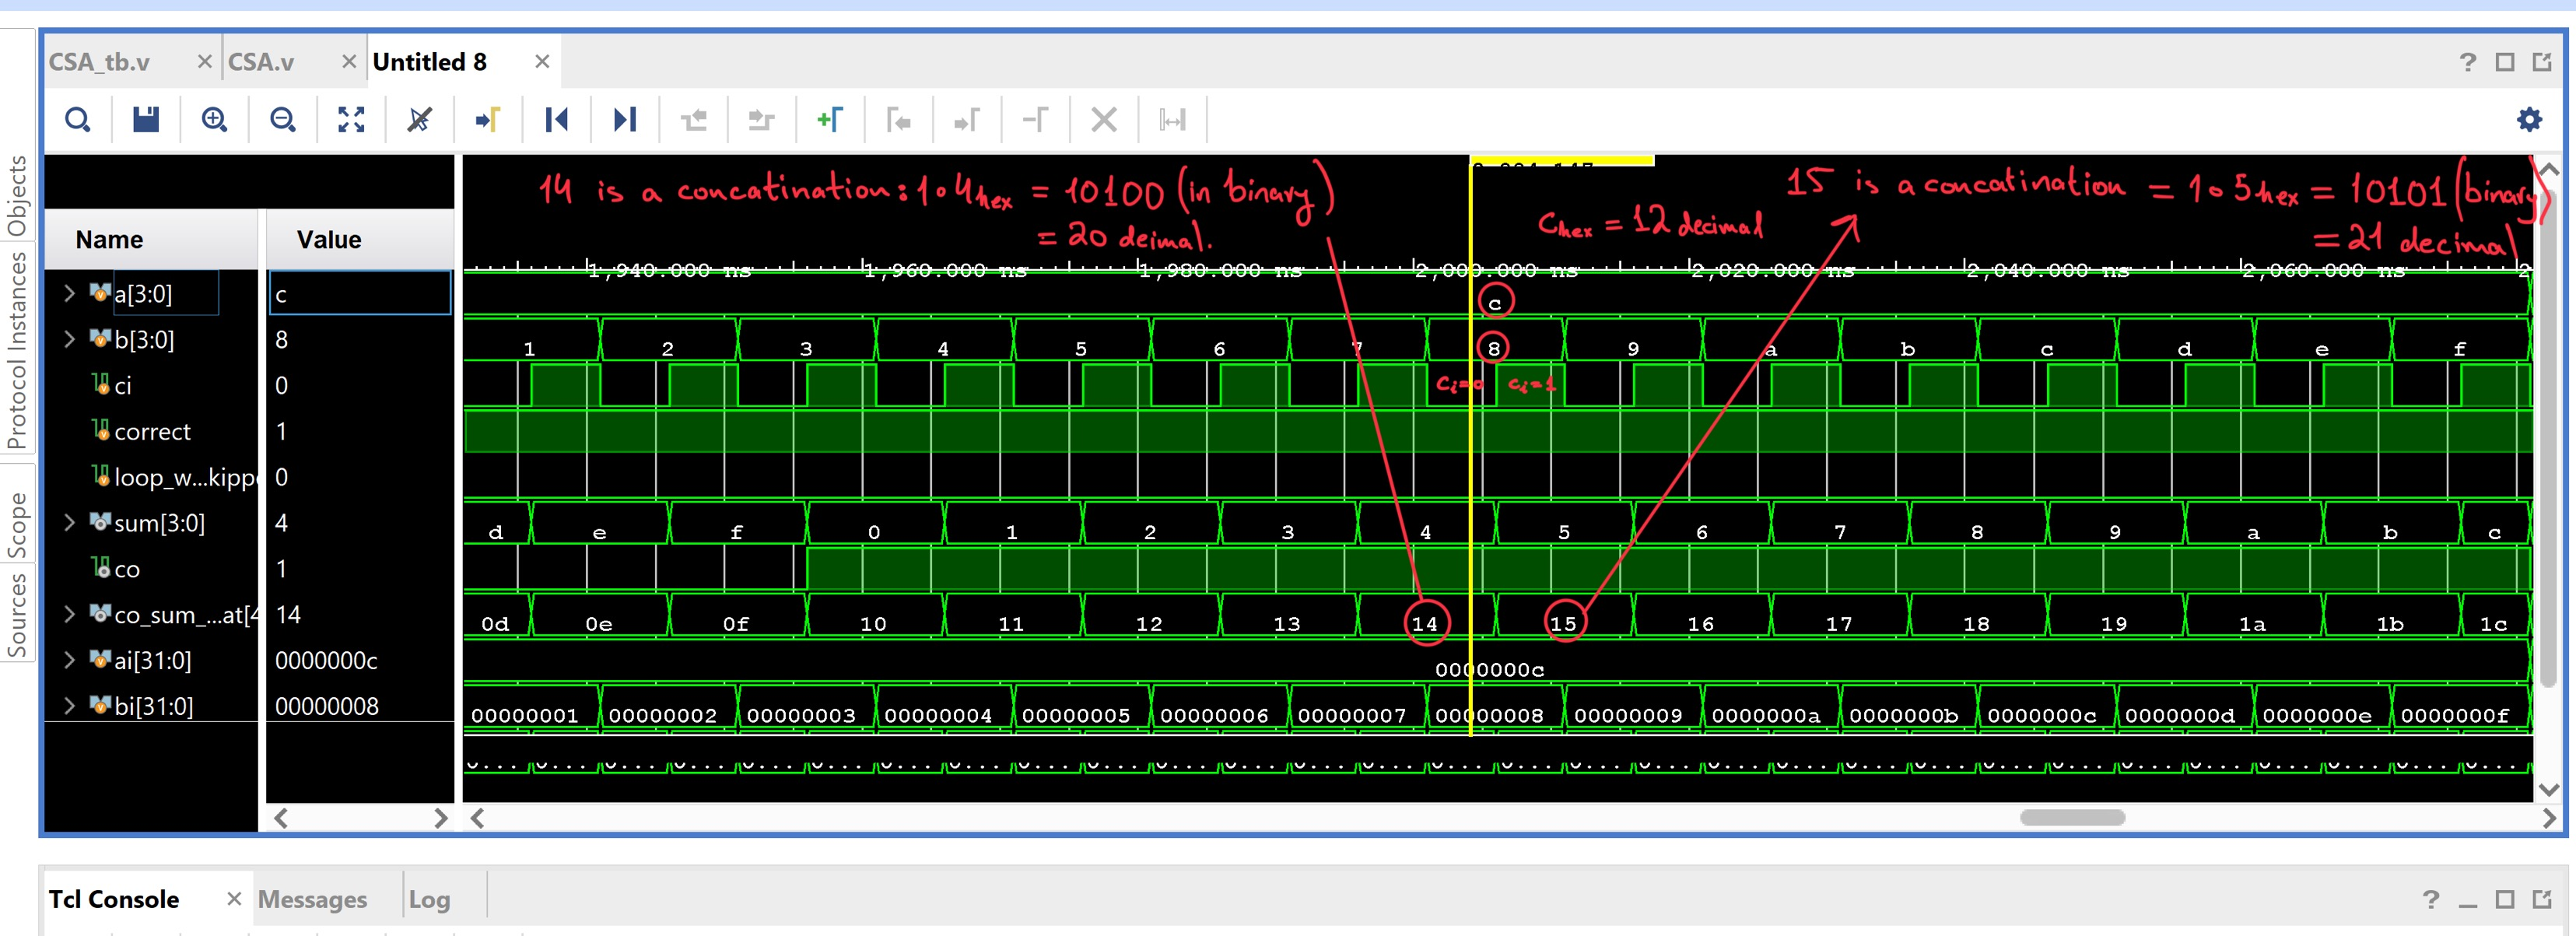
\includegraphics[width=1\linewidth]{CSA4-Annotated.jpg}
    \caption{CSA(4) Simulation Waveform (Annotated))}
    \label{fig:placeholder_csa(fignumber8)}
\end{figure}

%
% I should add here the CSA(4) Annotated 2
%
% Which must be Figure - 9


% =========================================================================
% ──  Section 3 - Limited Incrementor(Lim_Inc)─
% =========================================================================
\section{Limited Incrementor(Lim\_Inc)}

% =========================================================================
% ──  Sub-section 3.1 - Block Diagram─
\subsection{Block Diagram}
\noindent \textbf{Question:} Design a block diagram for the module, use instantiated modules, show and explain any other logic necessary.

\begin{figure}[H]
    \centering
    \fbox{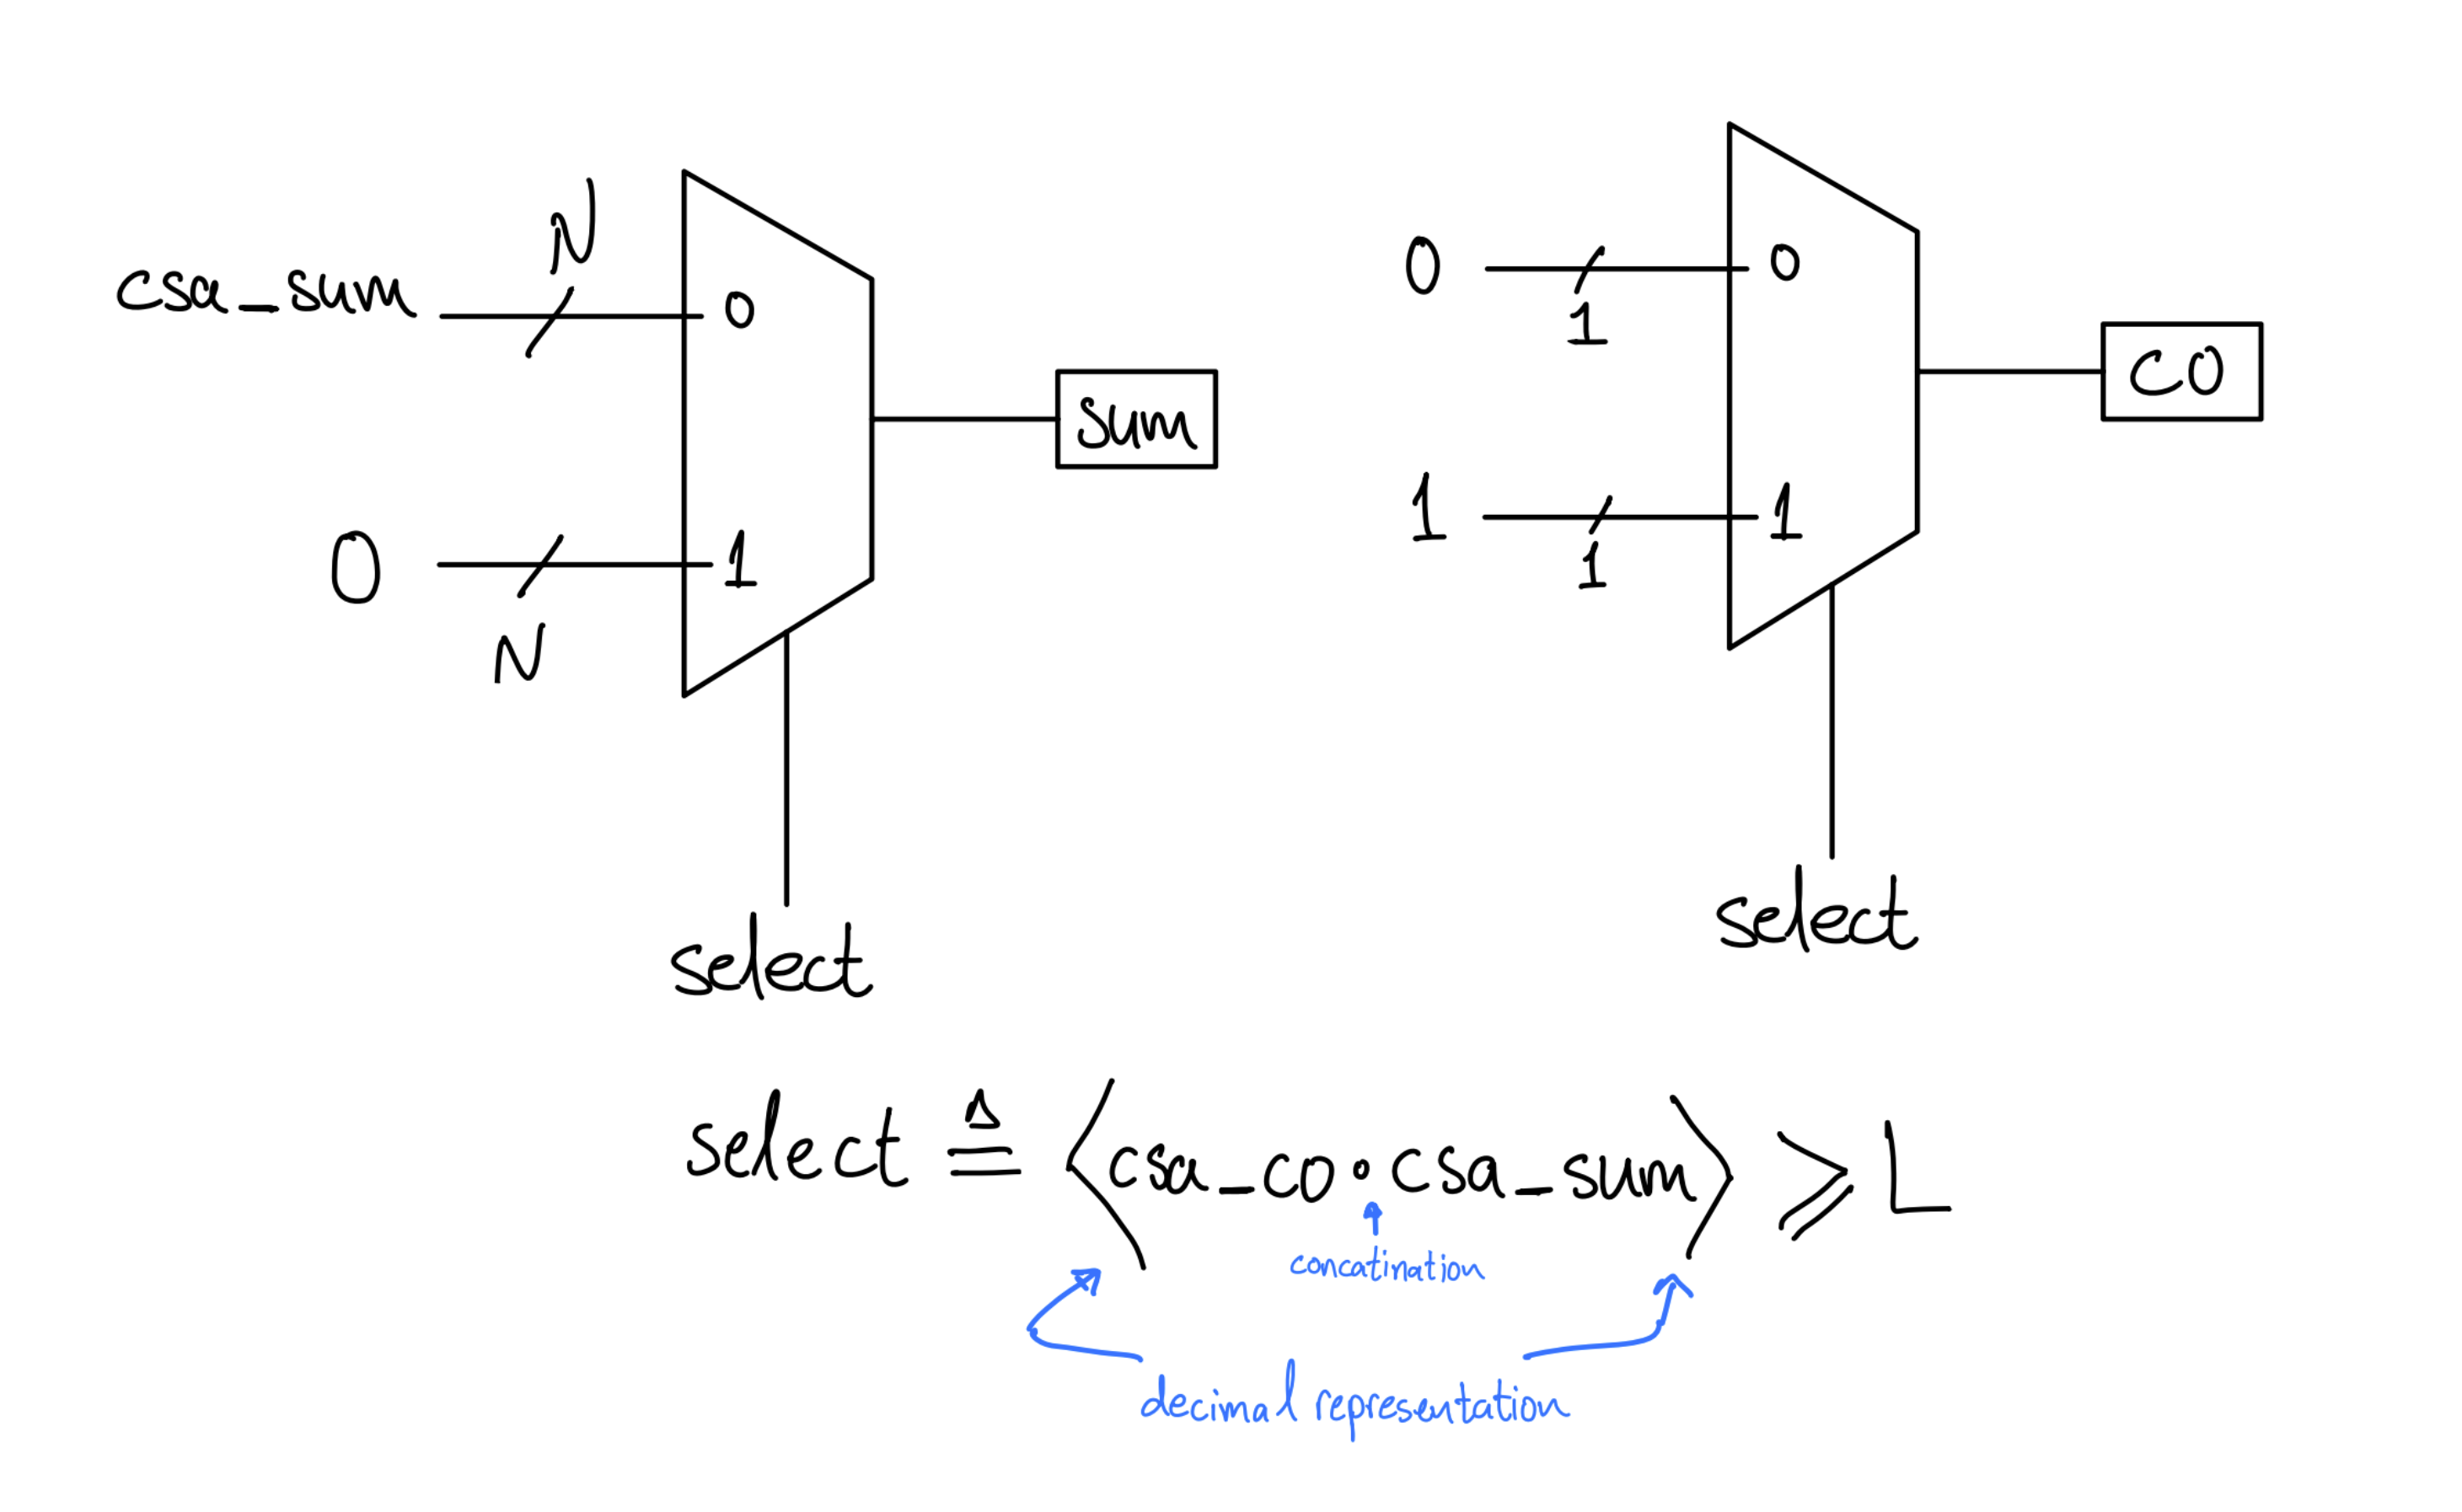
\includegraphics[width=1\linewidth]{Inc_Block_Diag2.png}}
    \caption{Limited Incrementor Block Diagram}
    \label{fig:placeholder_csa(fignumber10)}
\end{figure}

\noindent \textbf{Block Diagram Explanation:} The block diagram shows a pure conversion of the given functionality of the limited incrementer to logic. We begin by setting the selection channel to be a check if the following condition holds $\langle \text{csa}_{co} \circ \text{csa}_{\text{sum}} \rangle \ge L$, if it does (then selection = 1) then the circuit must output an N-bit length binary array of zeros as the sum, and a carry out bit that is equal to 1, which is the output of the two MUXes when they are outputting their "1" route.\\
Similarly, if the condition in the selection channel does not hold (i.e. select = 0), then the circuit must return the exact same input as the sum, and the carry out to be equal to 0, which is the output of the two MUXes when the are outputting their "0" route.





\newpage
\begin{figure}[h]
    \centering
    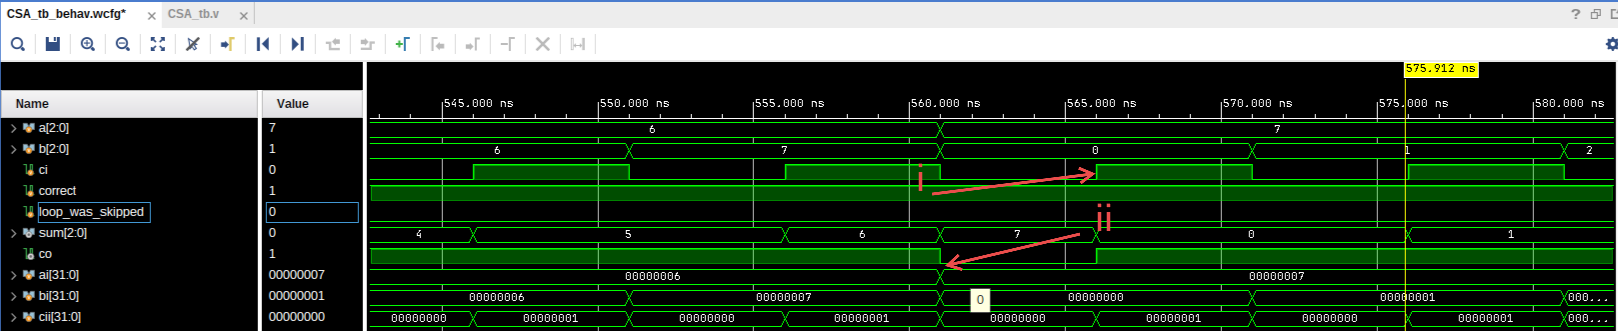
\includegraphics[width=\textwidth, height=5cm]{csa_new.png} 
    \caption{Zoomed in view of the simulation focusing on carry propagation.}
    \label{fig:csa_zoomed}
\end{figure}

\noindent In the waveform viewer we can see the value of each

\newpage
%%%%%%%%%%%%%%%%       S   T   I   T   I   A
%%%%%%%%%%%%%%%%%%     S   T   I   T   I   A
%%%%%%%%%%%%%%%%%%%%%  S   T   I   T   I   A
%%%%%%%%%%%%%%%%%%%%%%%S   T   I   T   I   A
%%%%%%%%%%%%%%%%%%%%%%%S   T   I   T   I   A
%%%%%%%%%%%%%%%%%%%%%  S   T   I   T   I   A
%%%%%%%%%%%%%%%%%%     S   T   I   T   I   A
%%%%%%%%%%%%%%%%       S   T   I   T   I   A
%
%
%start the debouncer and everything after part 6
%
%
\section{Debouncer}
 
\subsection{Block Diagram}
 
\noindent \textbf{Question:} Design a block diagram for the module, use instantiated modules, show and explain any other logic necessary.\\
 
\begin{figure}[h]
    \centering
    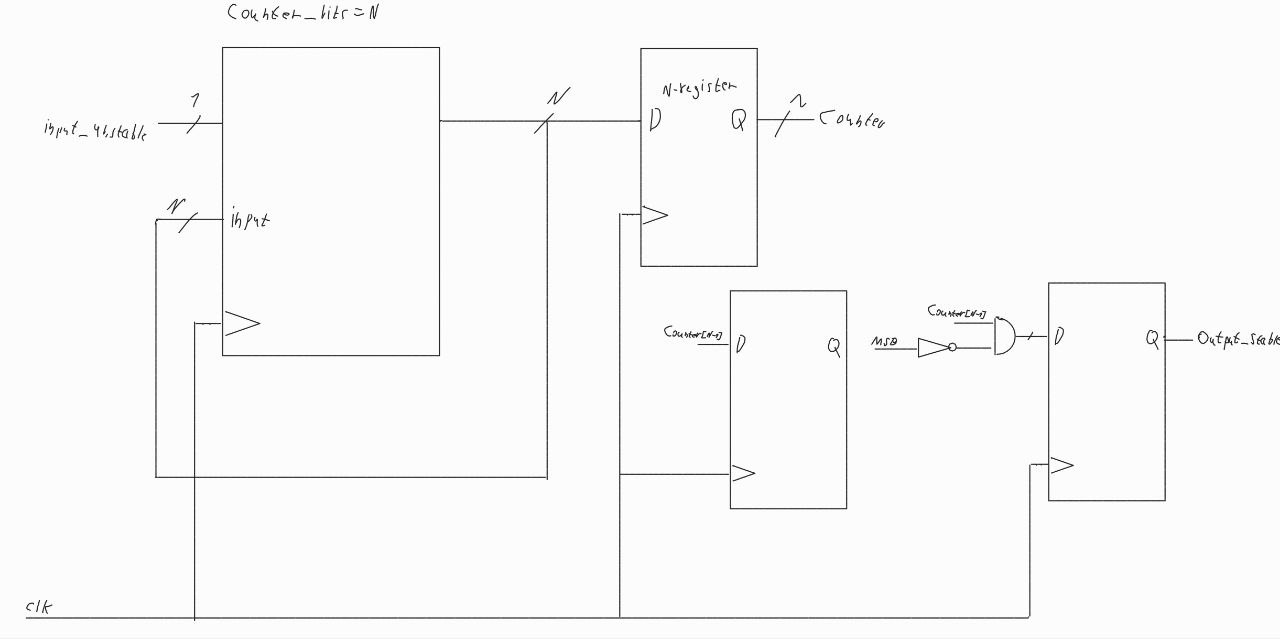
\includegraphics[width=0.9\linewidth]{debouncer_block_diagram.png}
    \caption{Debouncer Block Diagram}
    \label{fig:debouncer_bd}
\end{figure}

\noindent \textbf{Block Diagram Explanation:}
Our debouncer uses a saturated $N$-bit counter register, a single flip-flop, and an AND gate with one inverted input.\\On every rising clock edge, if\\ \texttt{input\_unstable} = 1 the counter increments , and if \texttt{input\_unstable} = 0 the counter decrements (saturating at 0). The flip-flop \texttt{msb} samples \texttt{counter[N-1]} on each clock edge, delaying the MSB by one cycle. The output is then:
\[
\texttt{output\_stable}(t) = \overline{\texttt{counter}[N{-}1](t{-}2)} \;\&\; \texttt{counter}[N{-}1](t{-}1)
\]
This implements a rising-edge detector on the counter's MSB: \texttt{output\_stable} goes high for exactly one clock cycle at the moment the MSB transitions from 0 to 1. This ensures a clean, single-cycle pulse regardless of how long the physical button is held.
 
\newpage
\subsection{Counter Value Tradeoff}
 
\noindent \textbf{Question:} Discuss the tradeoff between choosing high and low values for the counter, and how is this related to the low-pass-filter debouncing approach we saw in the previous experiments.\\
 
\noindent \textbf{Answer:}
The \texttt{COUNTER\_BITS} parameter determines the duration of the debounce interval. Increasing its value enlarges the counter, which improves immunity to noise and contact bouncing but also introduces longer latency before the system responds to a button press. Conversely, reducing this value shortens response time but increases the likelihood of false triggering caused by unstable or noisy input signals.\\\\This tradeoff is directly analogous to the low-pass-filter-based debouncing approach from earlier experiments. A lower cutoff frequency averages the input over a longer time, suppressing bouncing at the cost of increased delay, while a higher cutoff frequency allows faster response with reduced noise suppression. Similarly, a larger counter value requires longer input stability, whereas a smaller counter value reacts faster but is more sensitive to noise.
 
\newpage

\section{Seven Segment Display (Seg\_7\_Display)}
 
\subsection{Clock Division Selection}
 
\noindent \textbf{Question:} Describe your choice of bits for clock division and justify your answer analytically.\\
 
\noindent \textbf{Answer:}
The provided clock runs at 100\,MHz, so it ticks every 10\,ns.\\
The \texttt{clkdiv} register increments every clock cycle, so bit~$n$ toggles every $2^n$ cycles, i.e.\ every $10 \times 2^{n}$\,ns.\\
Since our design drives 4 digits, we need two bits to cycle through them. The total refresh time for all 4 digits must be between 1\,ms and 16\,ms to avoid visible blinking. If we select bits \texttt{[19:18]}, bit~18 changes every:
\[
10 \times 2^{18}\;\text{ns} = 2{,}621{,}440\;\text{ns} \approx 2.62\;\text{ms}
\]
The total refresh cycle for all four digits is then $4 \times 2.62 = 10.49$\,ms, which falls well within the required range of 1--16\,ms.

\newpage

\section{Stopwatch}
 
\subsection{Block Diagram}
 
\noindent \textbf{Question:} Design a block diagram for the module, use instantiated modules, show and explain any other logic necessary.
 
\begin{figure}[h]
    \centering
    \includegraphics[width=0.95\linewidth]{Stopwatch_block_diagram.png}
    \caption{Stopwatch Top-Level Block Diagram}
    \label{fig:stopwatch_bd}
\end{figure}
\newpage
 
\subsection{Elaborated Design Schematic}
 
 
\begin{figure}[h]
    \centering
    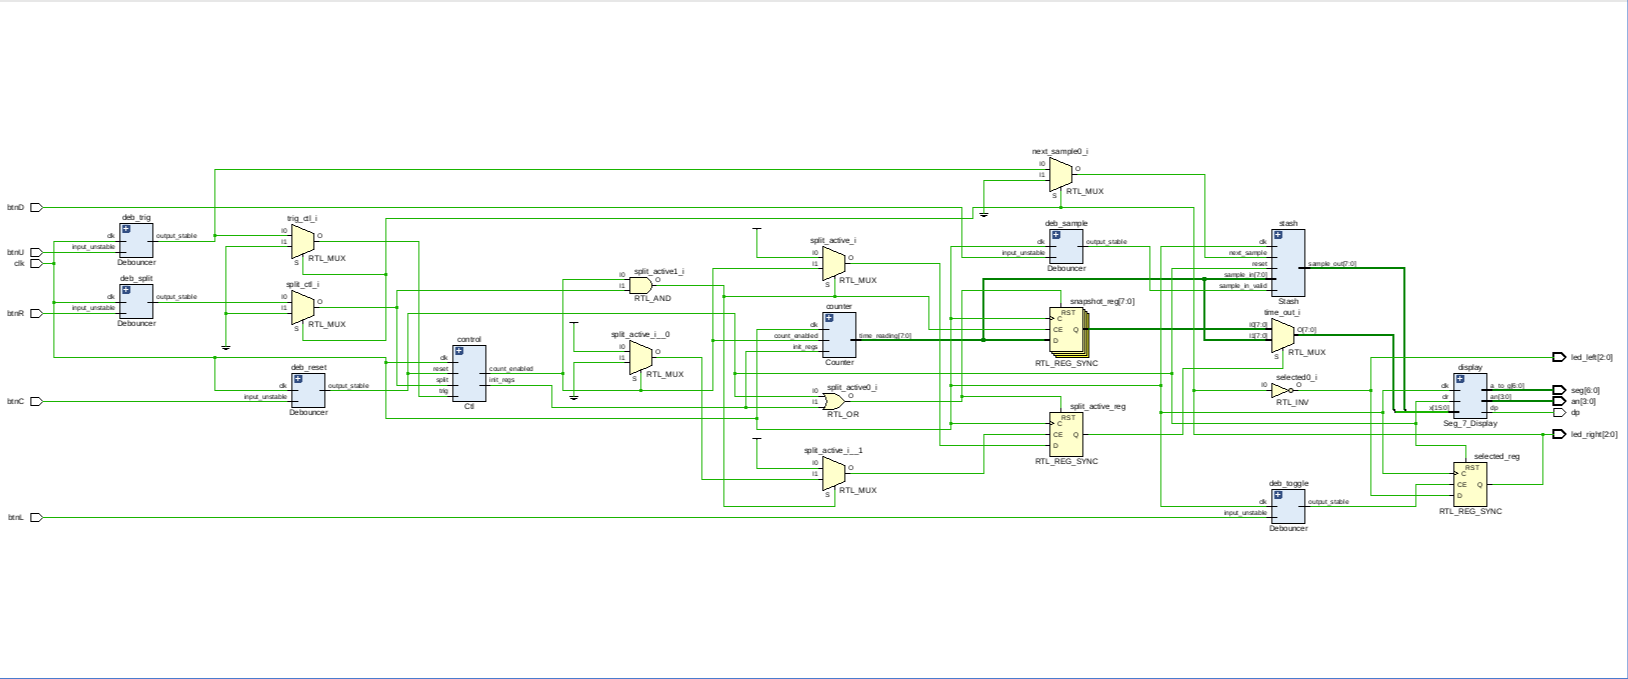
\includegraphics[width=\textwidth, angle=90]{stopwatch_e.png}
    \caption{Elaborated Design Schematic}
    \label{fig:stopwatch_elaborated}
\end{figure}
\noindent The elaborated design schematic shows all instantiated modules (5 Debouncers, Ctl, Counter, Stash, Seg\_7\_Display) with their correct interconnections. All top-level inputs (\texttt{btnC}, \texttt{btnU}, \texttt{btnR}, \texttt{btnL}, \texttt{btnD}, \texttt{clk}) and outputs (\texttt{seg}, \texttt{an}, \texttt{dp}, \texttt{led\_left}, \texttt{led\_right}) are present. The split logic and choose logic appear as MUXes and registers between the main modules.
\newpage

 
\subsection{Synthesized Design Comparison}
 
\begin{figure}[h]
    \centering
    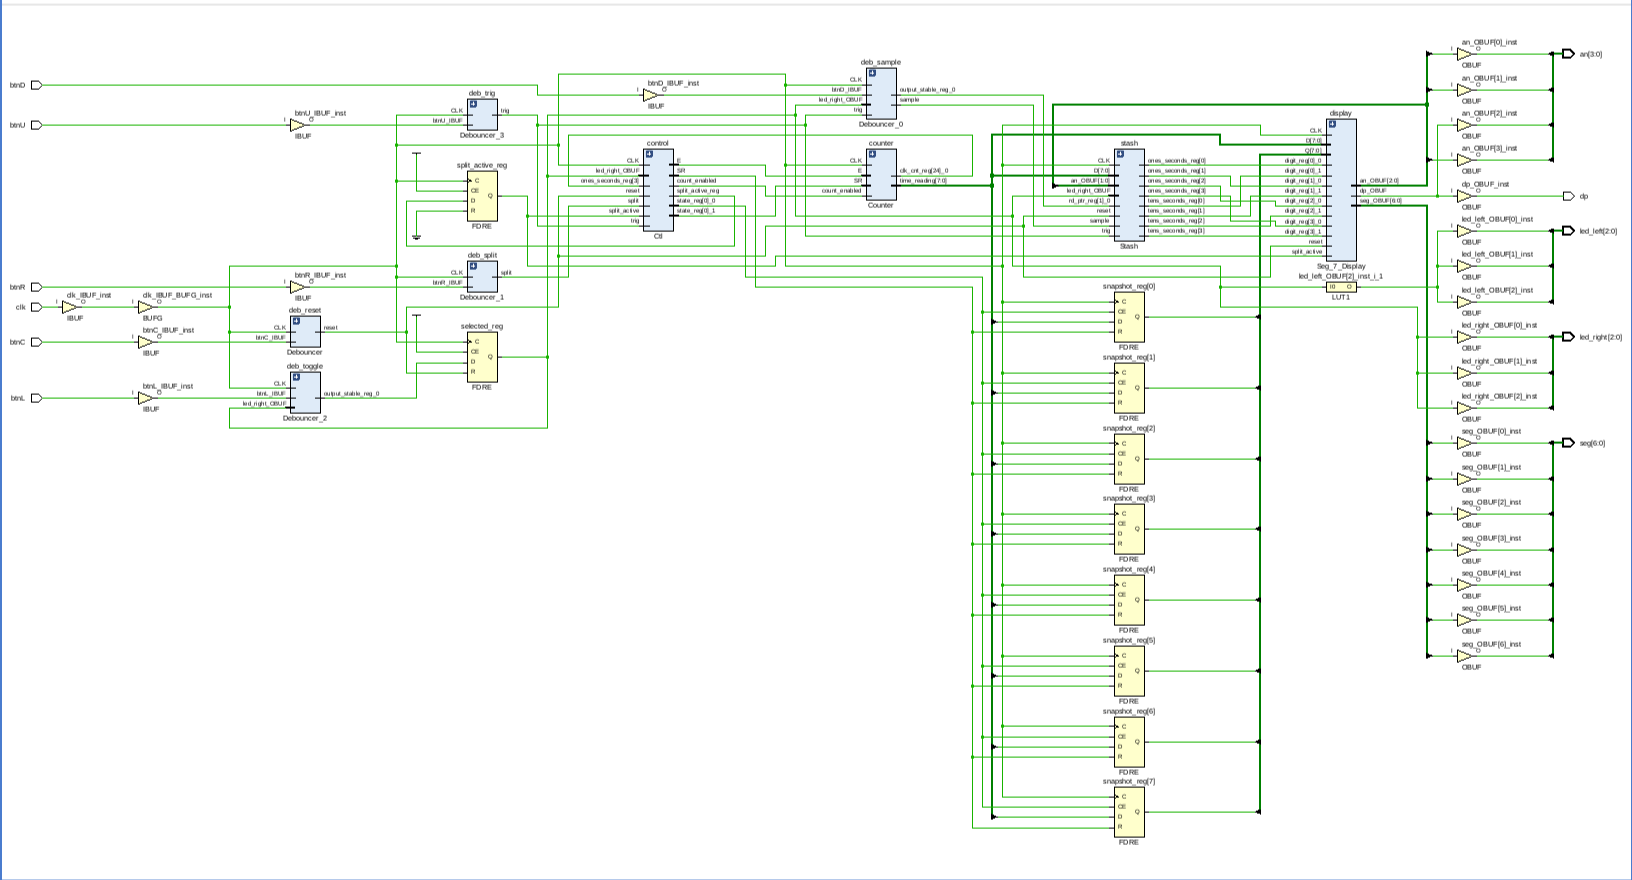
\includegraphics[width=\textwidth, height=14cm]{stopwatch_synthesized_design.png}
    \caption{Synthesized Design Schematic}
    \label{fig:stopwatch_synthesized}
\end{figure}
 
\noindent \textbf{Differences:}
In the elaborated design, we see the logical/behavioral structure as written in Verilog---high-level modules, generic RTL primitives (RTL\_MUX, RTL\_REG, RTL\_AND), and abstract signal buses. After synthesis, Vivado maps the design onto actual FPGA primitives: LUTs (Look-Up Tables), FDREs/FDSEs (flip-flops with reset/set and enable), IBUFs/OBUFs (I/O buffers), and a BUFG (global clock buffer). The synthesizer also performs optimizations such as merging logic, removing unused paths, and flattening hierarchies where beneficial.
 
 
\newpage


\section{Timing and summary}
\subsection{Timing Summary}
 
\noindent \textbf{Question:} Provide a screenshot of the design timing summary exhibiting positive slack for both setup and hold times.
 
\begin{figure}[h]
    \centering
    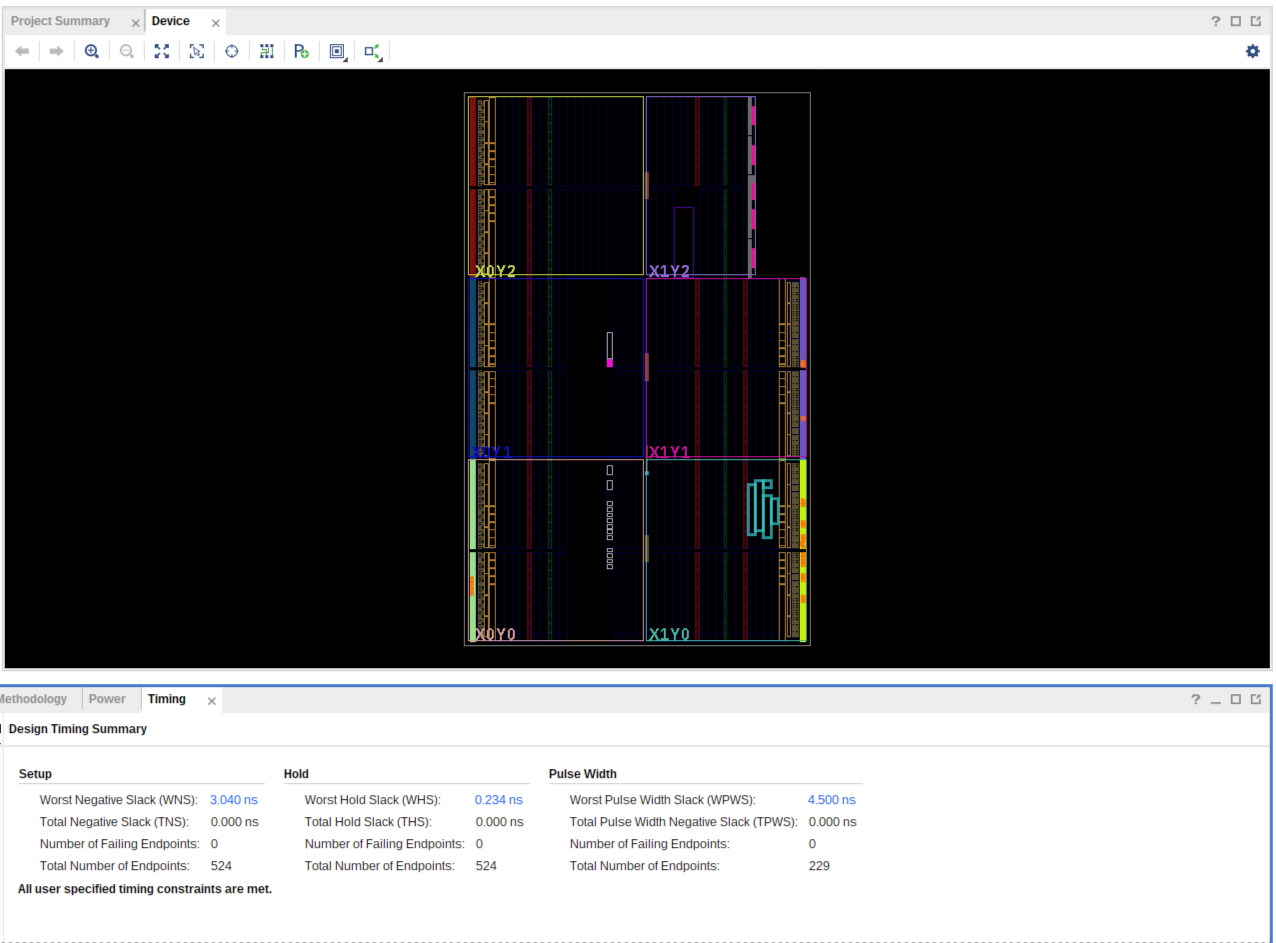
\includegraphics[width=\textwidth]{stopwatch_timing.png}
    \caption{Design Timing Summary --- all timing constraints are met.}
    \label{fig:timing_summary}
\end{figure}
\noindent As shown in the timing summary, all specified timing constraints are met:
\begin{itemize}
    \item \textbf{Setup:} Worst Negative Slack (WNS) = 3.040\,ns (positive $\Rightarrow$ constraint met)
    \item \textbf{Hold:} Worst Hold Slack (WHS) = 0.234\,ns (positive $\Rightarrow$ constraint met)
    \item \textbf{Pulse Width:} Worst Pulse Width Slack (WPWS) = 4.500\,ns (positive $\Rightarrow$ constraint met)
\end{itemize}
\newpage

 
\subsection{Critical Setup Path}
 setup path.
 
\begin{figure}[h]
    \centering
    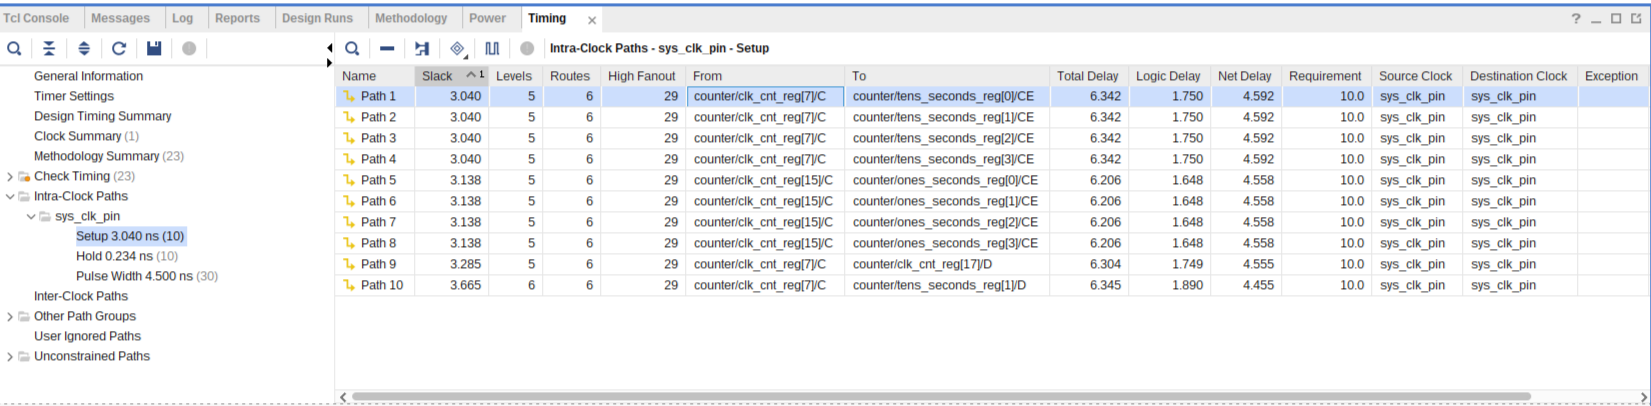
\includegraphics[width=\textwidth]{timing_setup.png}
    \caption{Setup timing paths (sorted by slack)}
    \label{fig:timing_setup}
\end{figure}
 
\noindent To calculate the critical (longest) path delay:
\[
longest path = clock\_period - setup\_min\_slack = 10\;\text{ns} - 3.040\;\text{ns} = 6.96\;\text{ns}
\]
From the detailed timing report (Figure~\ref{fig:timing_setup}),the critical path runs from\\ \texttt{clk\_cnt\_reg[7]/C} to \texttt{tens\_seconds\_reg[0]/CE}, with a total delay of 6.342\,ns .
 
\begin{figure}[h]
    \centering
    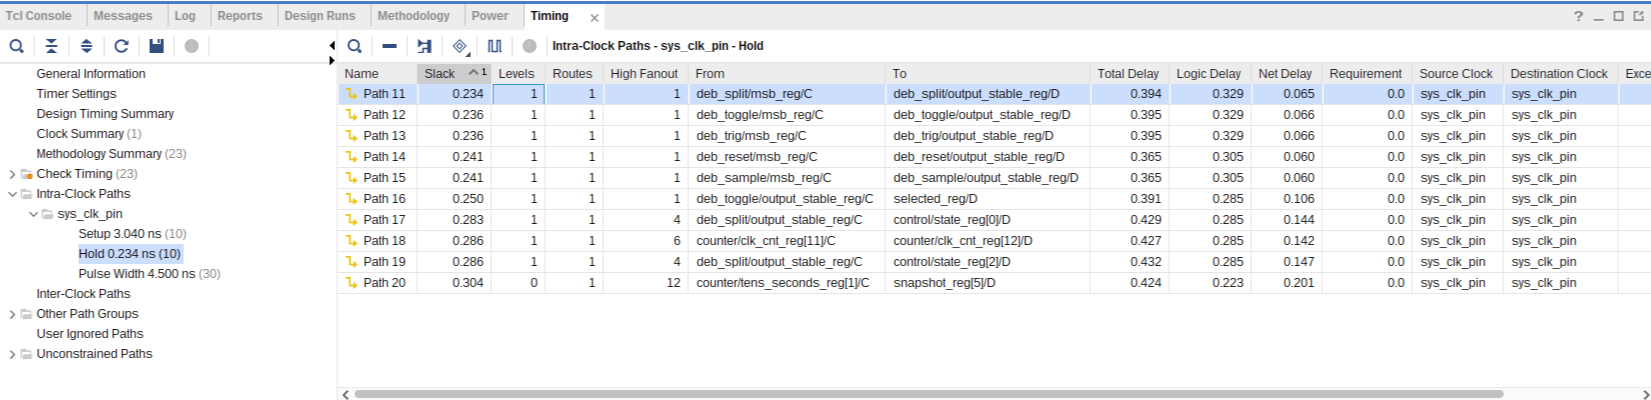
\includegraphics[width=\textwidth]{timing_hold.png}
    \caption{Hold timing paths (sorted by slack)}
    \label{fig:timing_hold}
\end{figure}
 
\noindent The hold timing paths (Figure~\ref{fig:timing_hold}) also show positive slack across all paths, confirming that the design meets hold time requirements as well.
 
 
\newpage
 
\subsection{Project Summary}
 
\noindent \textbf{Question:} Provide images of the working project.
 
\begin{figure}[h]
    \centering
    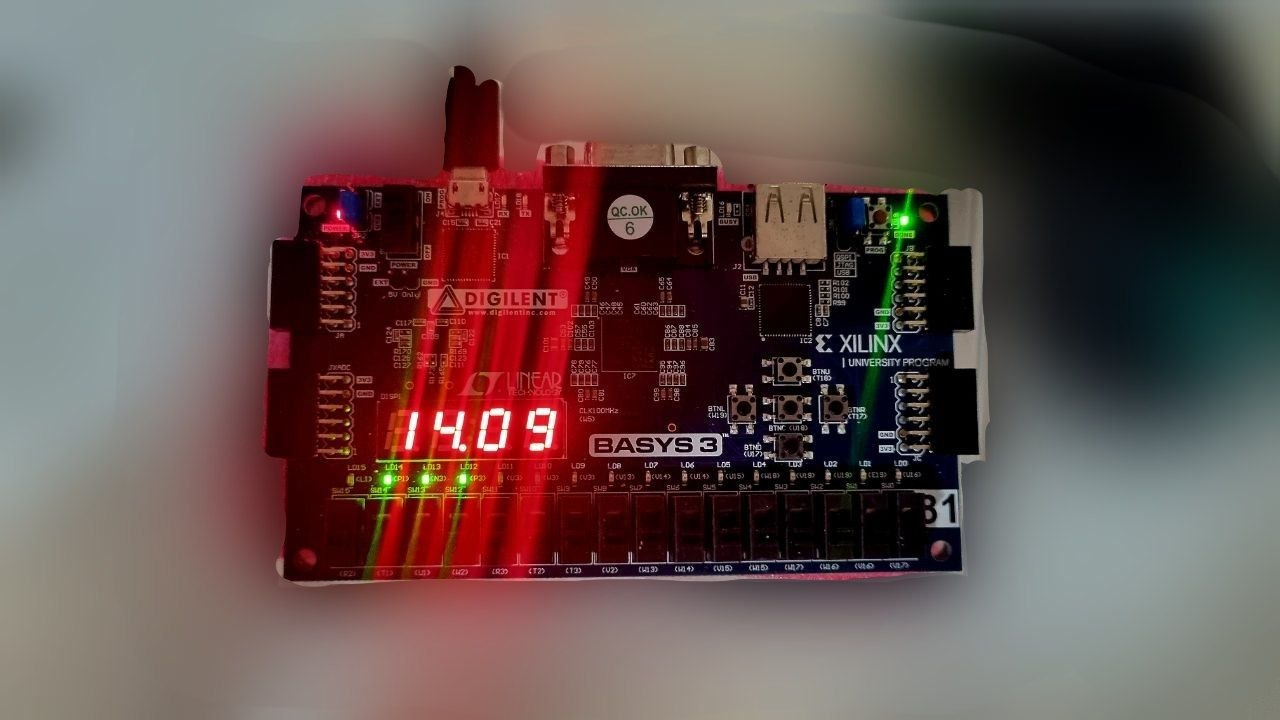
\includegraphics[width=\linewidth]{fpga_board_working.jpg}
    \caption{Working Stopwatch with stash on BASYS3 Board}
    \label{fig:working_board}
\end{figure}
 
 
\newpage
 
\end{document}